\section{Laufzeitsicht}
At least 1 UML sequence diagram of main scenario with explanation
Error and exception behaviour
\subsection{Account registrieren}

\subsection{Neuer Spieler importieren}

Um einen neuen Spieler zu importieren, wird eine Anfrage von dem Front and die "Player-API" gesendet.
Da diese Anfrage zustandslos ist, werden regelmäßig HTTP-Anfragen gesendet, um den aktuellen Import-Status
zu erhalten.
Diese Informationen werden im Frontend an den entsprechenden stellen dargestellt.
Im Player-API Service wird für den Import ein Backgroundtask gestartet, der über einen grpc Stream den Import im
Games Importer Service startet und die Anzahl der importierten Spiele streamt.

\graphic{cdc-07-import-player.drawio}{Flussdiagramm des Spieler imports}

\subsection{Spieler vergleichen}

Das Diagramm in Abbildung~\ref{fig:compare-diagram} stellt den Ablauf dar, wenn sich ein Spieler mit anderen Spielern vergleichen will.
\begin{figure}
    \centering
    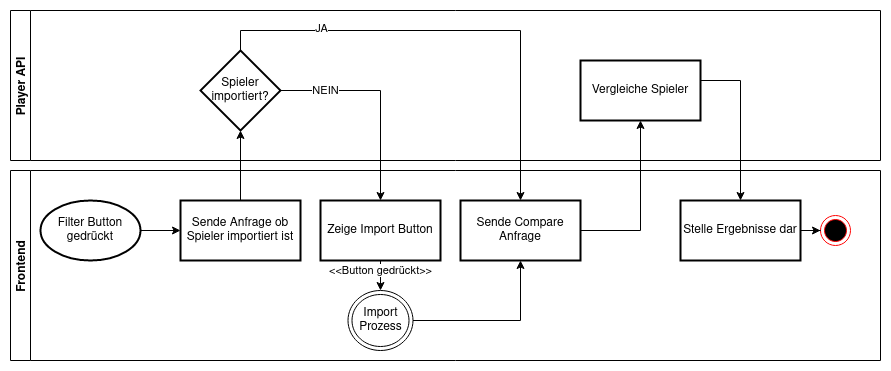
\includegraphics[width=\textwidth]{images/cdc-07-compare.drawio}
    \caption{Swimlane Diagramm zum Vergleich von Spielern}
    \label{fig:compare-diagram}
\end{figure}


\subsection{Error handling}
\subsubsection{Game importing}
\subsubsection{Monitoring}

Um die Applikation zu Monitoren werden verschiedene Tools verwendet.

\textbf{sentry} (\href{https://sentry.io/}{https://sentry.io/}) wird verwendet um Fehler zentral zu tracken und
Alerts zu verschicken.
Sentry wurde für alle Backend Services eingerichtet um einen Überblick über Serverseitiges Fehlverhalten zu bekommen.

Um die Performance von Requests zu tracken, wird \textbf{SigNoz} (\href{https://signoz.io/}{https://signoz.io/}) verwendet.
Damit werden Traces für Anfragen erstellt, womit festgestellt werden kann wie lange Anfragen brauchen und welche Methode wie lange braucht.
Außerdem werden automatisch Datenbank Operationen gemessen, wodurch es möglich ist zwischen Applikationslogik
und Datenbank Operationen zu unterscheiden, wie in Abbildung~\ref{fig:signoz-traces} zu sehen ist.
\begin{figure}
    \centering
    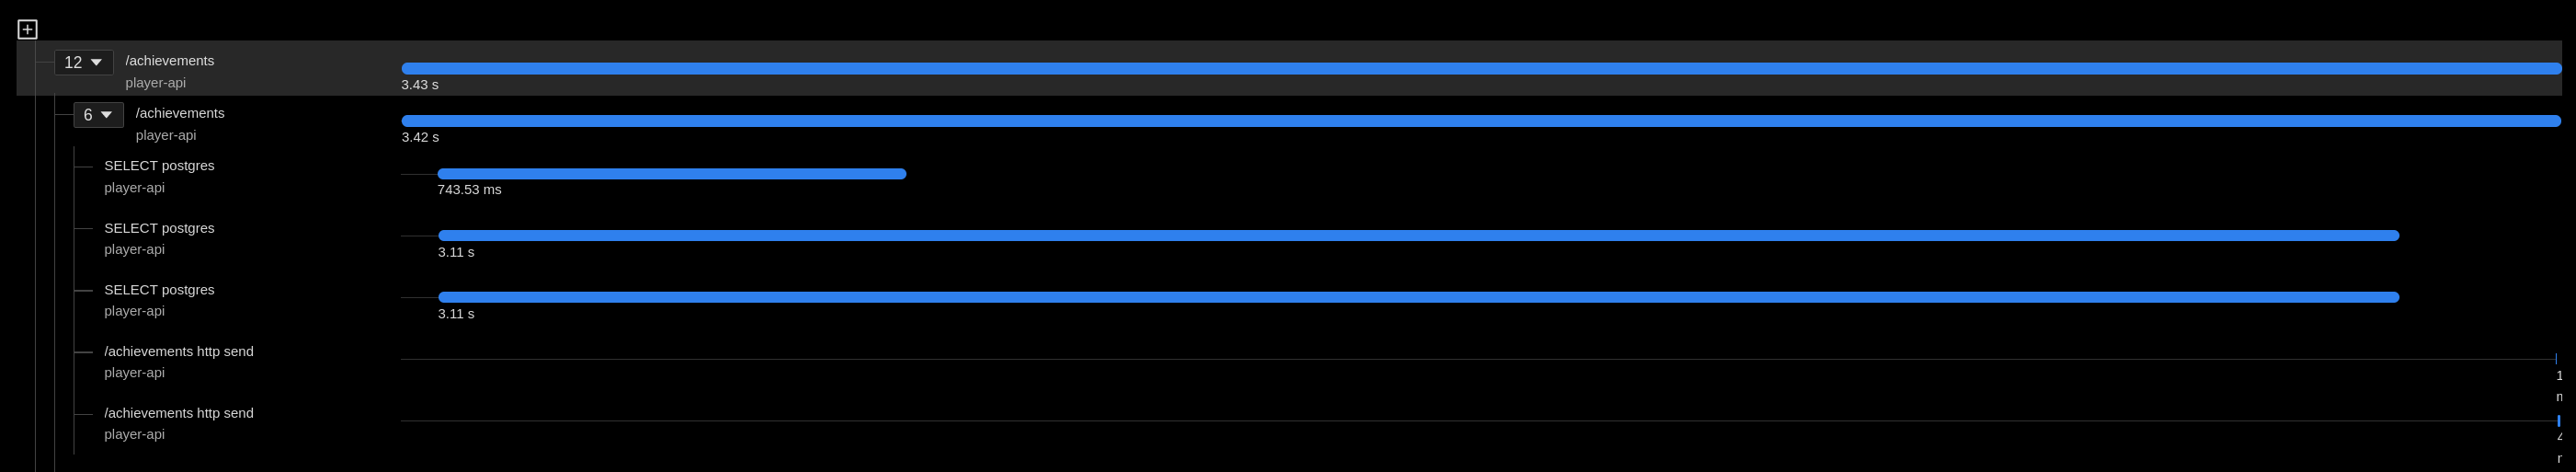
\includegraphics[width=\textwidth]{images/signoz_traces}
    \caption{Trace Details in SigNoz zu einem /achievements Request}
    \label{fig:signoz-traces}
\end{figure}